\documentclass{beamer}

\usecolortheme{orchid}

\usepackage{color}
\definecolor{darkred}{RGB}{180,0,0}

\usepackage{minted}

\title{Parsing and Reverse Engineering Binary Files}
\subtitle{Lessons learned...\newline{}\small{}so far...}
\author{Kenneth Nielsen (CINF)}
\institute
{
      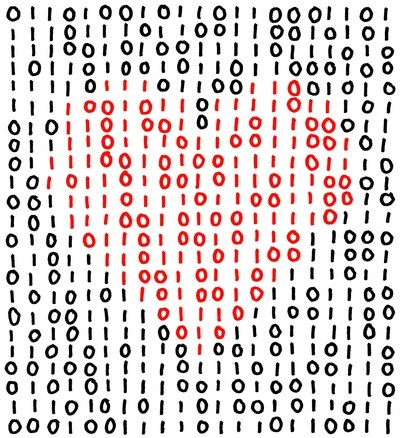
\includegraphics[width=0.25\textwidth]{binary_heart}\newline
      https://xkcd.com/99/
}
\date{
  Python and beers presentation,\\
  January 28, 2016}
\subject{Computer Science}

\AtBeginSection[]
{
  \begin{frame}<beamer>
    \frametitle{Outline}
    \tableofcontents[currentsection]
  \end{frame}
}

\begin{document}

\begin{frame}
  
\end{frame}

\frame{\titlepage}

%\section{About me}

\begin{frame}
  \frametitle{About me}
  \begin{itemize}
    \item My name is Kenneth Nielsen and I work at CINF
    \item Free and open source software (FOSS) enthusiast
    \item Use way too much time on Python conference presentations on
      youtube
  \end{itemize}
  \begin{block}{Slides and examples}
    \center
    \footnotesize
    \texttt{git clone https://github.com/KennethNielsen/presentations.git}\newline
    \newline
    \texttt{https://github.com/KennethNielsen/presentations}
    \texttt{http://bit.ly/1FclzDR}
  \end{block}
\end{frame}

\section{Introduction}

\begin{frame}
  \frametitle{Introduction}
  \begin{itemize}
  \item Parse binary file format, simpler format is unavailable
  \item E.g. pull data out of files created by instrument software
  \item With or without specification (emphasis is on without)
  \item More talk of techniques than code (though there is some at the end)
  \item Some talk about binary data in general
  \end{itemize}
\end{frame}

\section{What do I mean by binary file}

\begin{frame}
  \frametitle{What do I mean by binary file?}
  \begin{block}{The narrow definition}
    \begin{itemize}
    \item Not clear text e.g. XML, JSON or custom text format
    \item Simple binary files!
    \item Concatenation of binary representation of values
    \item No type information
    \item No third party serialization
    \end{itemize}
  \end{block}
\end{frame}

\begin{frame}
  \frametitle{Binary representation of data}
  \begin{block}{It's all bits}
    \begin{itemize}
    \item Computers only know about bits (1000101010111010101)
    \item The \textbf{type} of the data is what gives the bits meaning (converts it to a \textbf{value})
    \item For the values, one or more bytes can be used, depending on the requirements
    \end{itemize}
  \end{block}
  Examples of data types are:
  \begin{itemize}
  \item Signed and unsigned integers: short (int8), unsigned long (uint64)
  \item Booleans (commonly a special case of a 1 byte integer)
  \item Floats and doubles: 4 or 8 bytes floating point numbers
  \item Strings..!
  \end{itemize}
\end{frame}

\begin{frame}
  \frametitle{Strings}
  1 min in bytes and encodings (which is really a presentation on its own)
  \begin{block}{We can only store bytes}
    \begin{itemize}
    \item Text is stored in an encoding
    \item Many (all?) encoding contains ASCII at the first 128 positions
    \item Which means that it is recognizable
    \item After parsing, bytes should be decoded
    \item Some encodings are fixed width other variable
    \item Sometimes the string is prefixed with the number of bytes
    \item It's a pain
    \end{itemize}
  \end{block}
\end{frame}

\begin{frame}[fragile]
  \frametitle{Endianness}
  \begin{alertblock}{The order of bytes in multi byte types}
    To make matters worse, different ``computer'' architectures does
    not agree on in which order bytes in a multi-byte type should be
    stored!\newline
    \newline
    \textbf{This is referred to as the ``endianness''}
  \end{alertblock}
  \vspace{0.5cm}
  \small
  From wikipedia: https://en.wikipedia.org/wiki/Endianness\newline
  \begin{quotation}
    With big-endian the most significant byte of a word is stored at a
    particular memory address and the subsequent bytes are stored in
    the following higher memory addresses, the least significant byte
    thus being stored at the highest memory address. Little-endian
    format reverses the order and stores the least significant byte at
    the lower memory address with the most significant byte being
    stored at the highest memory address
  \end{quotation}
\end{frame}

\begin{frame}[fragile]
  \frametitle{One set of bytes, many meanings}
  \scriptsize
  \begin{minted}{text}
    The bytes ['0x50', '0x79', '0x74', '0x68', '0x6f', '0x6e', '0x20', '0xFF']
                   char[] : b'Python \xff'
    Not relevant     int8 : (80, 121, 116, 104, 111, 110, 32, -1)
    Not relevant    uint8 : (80, 121, 116, 104, 111, 110, 32, 255)
    Little-Endian   int16 : (31056, 26740, 28271, -224)
    Big-Endian      int16 : (20601, 29800, 28526, 8447)
    Little-Endian  uint16 : (31056, 26740, 28271, 65312)
    Big-Endian     uint16 : (20601, 29800, 28526, 8447)
    Little-Endian   int32 : (1752463696, -14651793)
    Big-Endian      int32 : (1350136936, 1869488383)
    Little-Endian  uint32 : (1752463696, 4280315503)
    Big-Endian     uint32 : (1350136936, 1869488383)
    Little-Endian   int64 : (-62928970010298032,)
    Big-Endian      int64 : (5798793987111133439,)
    Little-Endian  uint64 : (18383815103699253584,)
    Big-Endian     uint64 : (5798793987111133439,)
    Little-Endian   float : (4.6179809698425413e+24, -2.1324988332749138e+38)
    Big-Endian      float : (16740622336.0, 7.369732216716093e+28)
    Little-Endian  double : (-2.2536157545457443e+304,)
    Big-Endian     double : (4.715928068041943e+79,)
  \end{minted}
  \normalsize
  There are 19 lines here! Luckily, often the endianness is known, which reduces it to 11
\end{frame}

\section{Tools for the job}
\begin{frame}
  \frametitle{The hex editor}
  \begin{block}{Your friend, the hex editor}
    \begin{itemize}
    \item At first intimidating and difficult to make sense of
    \item Then ... \textbf{incredibly} useful
    \end{itemize}  
  \end{block}
  \huge
  \vspace{2cm}
  DEMO ghex
\end{frame}

\begin{frame}
  \frametitle{The \texttt{struct} module}
  3 module functions:\newline
  \begin{itemize}
  \item \texttt{unpack(fmt, string)}
  \item \texttt{pack(fmt, v1, v2, ...)}
  \item \texttt{calcsize(fmt)}
  \end{itemize}
  make up the core of the functionality\newline
  \newline
  Most of the time we will just be using \texttt{unpack}.
  \vspace{1cm}
  \huge\newline
  DEMO in the terminal!
\end{frame}

\begin{frame}[fragile]
  \frametitle{With a format specification}
  Edited version of the specification of the \AA{}rhus type STM file format: http://owww.phys.au.dk/spm/programs/
  \footnotesize
  \begin{minted}{pascal}
    // Each image consists of a label record defined as follows:
    la=
    record
      //size in blocks, xch,ych are x,y pixels.
      nr,size,xch,ych,zch:smallint;
      //In Turbo Pascal format (year, month, day, hour, min, sec in 16
      //bit integers)
      time:datetime;
      xsize,ysize,xshift,yshift,zscale,tilt:smallint;
      speed:word; { now time in 10mS units 921221 S3 vers 6}
      // bias is -+10V for +-32 k  current is in 0.01 nA units
      bias,current:smallint;
      sample,title:string[20];
      postpr,postd1,constheight, { 910110 -constheight/postd2- }
      Currfac,R_Nr:smallint; { 930118 -Currfac/min- 931009 -R_Nr/max- }
      unitnr:smallint;  { 890612 }
      version:smallint;
      spare:array[48..63] of smallint;
    end;
  \end{minted}
\end{frame}

\begin{frame}[fragile]
  \frametitle{With a format specification}
  \begin{itemize}
  \item Depending on the implementation language, figure out what the integer names means
  \item By use of the specification, build up the formats
  \item Parse with \texttt{struct.unpack}
  \end{itemize}
\end{frame}

\begin{frame}
  \frametitle{Without a format specification}
  Look for information anywhere you can find it:
  \begin{itemize}
  \item (Half) implementations on the internet
  \item Possibly in other languages
  \item Online discussions
  \end{itemize}
  Some information is much better than no information.\newline
  \newline
  \textbf{Other than that, hang on tight for the rest of the ride.}
\end{frame}

\section{Typical anatomy of a binary file}
\begin{frame}[fragile]
  \frametitle{Typical anatomy of a binary file}
  \begin{columns}[onlytextwidth]
    \begin{column}{0.4\textwidth}
      A binary file may have a layout as:
      \begin{itemize}
      \item For multipart files, an index
      \item A header (metadata)
      \item The data
      \end{itemize}
    \end{column}
    \begin{column}{0.6\textwidth}
      \begin{minted}{text}
        Multipart     Single part

        +--------+    +--------+
        | Index  |    | Header |
        |--------|    |--------|
        |Header 1|    |        |
        |Data 1  |    |  Data  |
        |--------|    |        |
        |Header 2|    +--------+
        |Data 2  |
        +--------+
      \end{minted}
    \end{column}
  \end{columns}
\end{frame}

\begin{frame}[fragile]
  \frametitle{Empty space}
  \begin{columns}[onlytextwidth]
    \begin{column}{0.4\textwidth}
      The header may be sparse, with padding (of zero bytes) in between information items
    \end{column}
    \begin{column}{0.6\textwidth}
      \begin{minted}{text}
        +----------------+
        |ID14....Comment.|
        |....x-axis unit.|
        |................|
        |.Date...........|
        |......95365.....|
        +----------------+
      \end{minted}
    \end{column}
  \end{columns}
\end{frame}

\section{Parsing the data}

\begin{frame}
  \frametitle{Get an export of the data file}
  \begin{alertblock}{Get an export of any kind}
    Although the purpose of the exercise is to be able to read the
    binary files directly, having an export of both data and metadata
    for a few files to compare with is invaluable (maybe
    indispensable)\newline
    \newline
    From this export extract information about the number of data points
    and as much metadata as possible
  \end{alertblock}
\end{frame}


\begin{frame}[fragile]
  \frametitle{Finding the data}
  \begin{columns}[onlytextwidth]
    \begin{column}{0.5\textwidth}
      \begin{itemize}
      \item Use the hex editor
      \item In the case of a sparse header, look for when the data becomes
        dense and repeats in a pattern
      \item In the case of a dense header, without any clear start of
        data, calculate backwards from the end with the maximum number of
        bytes per point
      \end{itemize}
    \end{column}
    \begin{column}{0.5\textwidth}
      \begin{minted}{text}
        +----------------+
        |ID14....Comment.|
        |....x-axis unit.|
        |................|
        |.Date...........|
        |................|
        |................|
        |....3761....9578|
        |....7A74....8943|
        |....5679....9578|
        |....6899....7536|
        |....5478....1234|
        +----------------+
      \end{minted}
    \end{column}
  \end{columns}
\end{frame}

\begin{frame}
  \frametitle{Analyze (Important)}
  \begin{itemize}
  \item Measure how many bytes of data there is per point
  \item Is both x and y saved (xxxyyy or xyxyxy), or only y
  \item \textbf{NOTE:} That the data in the file, does not need to
    correspond to the expected data directly
  \item It may be scaled e.g. ADC integers instead of floats
  \item Compare with the export and see if there is a consistent
    scaling factor (or linear scaling relation)
  \end{itemize}
\end{frame}

\begin{frame}
  \frametitle{Quick detour on file objects}
  When working with text:
  \begin{itemize}
  \item \texttt{fileobject.read()}    Read it all
  \item \texttt{for line in fileobject:}    Iterate over lines in the file
  \end{itemize}
  But fileobject also have a ``cursor'', which is really useful. When
  working with binary data:
  \begin{itemize}
  \item \texttt{fileobject.read(n)}    Read n bytes
  \item \texttt{fileobject.seek(n, origin)}    Seek to byte n from origin
  \item \texttt{fileobject.tell()}    Get current position
  \end{itemize}
\end{frame}

\begin{frame}[fragile]
  \frametitle{Read until there is no more}
  \begin{minted}{python}
    data = []
    with open('FID1A.ch', 'rb') as file_:
        file_.seek(6144)
        raw = file_.read(8)
        while len(raw) == 8:
            data.append(unpack('<d', raw)[0])
            raw = file_.read(8)
    points = numpy.array(data)    
  \end{minted}
\end{frame}

\begin{frame}[fragile]
  \frametitle{Calculate number of points beforehand}
  \begin{minted}{python}
    with open('FID1A.ch', 'rb') as file_:
        file_.seek(0, 2)  # Seek to the end of the file
        end = file_.tell()
        num_points = (end - 6144) // 8
        file_.seek(6144)
        raw = file_.read(end - 6144)
        data = unpack('<{}d'.format(num_points), raw)
    points = numpy.array(data)
  \end{minted}
\end{frame}

\begin{frame}[fragile]
  \frametitle{Parse directly into numpy array}
  \begin{minted}{python}
    with open('FID1A.ch', 'rb') as file_:
        file_.seek(0, 2)  # Seek to the end of the file
        end = file_.tell()
        num_points = (end - 6144) // 8
        file_.seek(6144)
        points = numpy.fromfile(file_, dtype='<d',
                                count=num_points)
  \end{minted}
  \vspace{1cm}
  \huge DEMO data.py
\end{frame}

\section{Parsing the header}
\begin{frame}
  \frametitle{The big ``Can you spot the number in the big pile of numbers'' game}
  \LARGE
  \begin{block}{Look for know metadata items from your export by:}
  \begin{itemize}
  \item Use of a hex editor
  \item Searching for it by brute force
  \item Changing just one settings and look for differences in similar headers
  \end{itemize}    
  \end{block}
\end{frame}

\begin{frame}[fragile]
  \frametitle{Brute force search}
  \small
  \begin{minted}{python}
def find_number(value, filename, header_end, endiannes='>'):
    """Look for value in file named filename"""
    if isinstance(value, float):
        formats = 'fd'
    else:
        formats = 'bBhHiIqQ'

    with open(filename, 'rb') as file_:
        for index in range(header_end):
            for format_ in formats:
                file_.seek(index)
                raw = file_.read(calcsize(format_))
                value_at_index = \
                    unpack(endiannes + format_, raw)[0]
                if equal_or_close(value, value_at_index):
                    print('YATZY! Found value {} at index {}'.\
                          format(value, index))
  \end{minted}
  \LARGE DEMO header\_tools.py
\end{frame}


\begin{frame}[fragile]
  \frametitle{Look for differences, part1}
  \small
  \begin{minted}{python}
def bytes_diff(filename1, filename2, header_end):
    """Calculate bytes diff"""
    # Get the bytes
    byte_strings = []
    for filename in [filename1, filename2]:
        with open(filename, 'rb') as file_:
            byte_strings.append(file_.read(header_end))
  \end{minted}
\end{frame}

\begin{frame}[fragile]
  \frametitle{Look for differences, part2}
  \small
  \begin{minted}{python}
    start_pos = None
    diff1, diff2 = b'', b''
    for index, (byte1, byte2) in enumerate(zip(*byte_strings)):
        # In Python 3, iterating over bytes gives you numbers!
        if sys.version_info.major == 3:
            byte1, byte2 = bytes([byte1]), bytes([byte2])
        # Compare
        if byte1 != byte2:
            if start_pos is None:
                start_pos = index
            diff1 += byte1
            diff2 += byte2
        else:
            if start_pos is not None:
                print('At index:', start_pos)
                print(repr(diff1) + '\n' + repr(diff2) + '\n')
                start_pos = None
                diff1, diff2 = b'', b''
  \end{minted}
  \LARGE DEMO header\_tools.py
\end{frame}

\begin{frame}[fragile]
  \frametitle{Parse the header, part 1, table of fields}
  \small
  \begin{minted}{python}
fields = (
    ('sequence_line_or_injection', 252, UINT16),
    ('injection_or_sequence_line', 256, UINT16),
    ('start_time', 282, 'x-time'),
    ('end_time', 286, 'x-time'),
    ('version_string', 326, 'utf16'),
    ('description', 347, 'utf16'),
    ('sample', 858, 'utf16'),
    ('operator', 1880, 'utf16'),
    ('date', 2391, 'utf16'),
    ('inlet', 2492, 'utf16'),
    ('instrument', 2533, 'utf16'),
    ('method', 2574, 'utf16'),
    ('software version', 3601, 'utf16'),
    ('software name', 3089, 'utf16'),
    ('software revision', 3802, 'utf16'),
    ('units', 4172, 'utf16'),
    ('detector', 4213, 'utf16'),
    ('yscaling', 4732, ENDIAN + 'd')
)
  \end{minted}
\end{frame}

\begin{frame}[fragile]
  \frametitle{Parse the header, part 2}
  \small
  \begin{minted}{python}
def parse_header(file_):
    metadata = {}
    # Parse all metadata fields
    for name, offset, type_ in fields:
        file_.seek(offset)
        if type_ == 'utf16':
            metadata[name] = parse_utf16_string(file_)
        elif type_ == 'x-time':
            metadata[name] =\
                unpack(ENDIAN + 'f', file_.read(4))[0] / 60000
        else:
            metadata[name] =\
                unpack(type_, file_.read(calcsize(type_)))[0]

    # Convert date
    metadata['datetime'] = time.strptime(metadata['date'],
                                         '%d-%b-%y, %H:%M:%S')
    return metadata
  \end{minted}
  \LARGE DEMO header.py
\end{frame}

\begin{frame}
  \frametitle{That's it}
  The file is now parsed and we know something about how to read binary files!
  \vspace{0.5cm}
  \begin{alertblock}{Resist the temptation}
    Some of you may at this point feel an itching to try and
    \textit{make} a binary format of your own i.e. write binary files
    instead of reading them, because it somehow feel like the
    \textit{right} way to store stuff. \textbf{DON'T!!!}.\newline
    
    Wide use of custom format binary files is mostly a thing of the
    past. In the year 2016 custom format binary should \textbf{only}
    be used if it is absolutely necessary. Most things can be handled
    by simply using two files, one for the numpy data (which can write
    itself) and one of the metadate e.g. in JSON. If you really need a
    single file format with high space and read/write efficiency look
    into HDF5.
  \end{alertblock}
\end{frame}

\section{Summary}
\begin{frame}
  \frametitle{Summary, tools}
  \begin{itemize}
  \item A hex editor
  \item Struct
  \end{itemize}
\end{frame}

\begin{frame}
  \frametitle{Summary, anatomy}
  \begin{itemize}
  \item Header
  \item Data
  \item Possibly an index, for multipart files
  \end{itemize}
\end{frame}

\begin{frame}
  \frametitle{Summary, data}
  \begin{itemize}
  \item Look for data with hex editor
  \item Calculate backwards from the known number of points
  \item Parse with struct
  \item Or directly into numpy.array
  \end{itemize}
\end{frame}

\begin{frame}
  \frametitle{Summary, header (metadata)}
  \begin{itemize}
  \item Look for fields with hex editor
  \item Search for known numbers
  \item Look at differences
  \item Write out a table of known fields
  \item Parse with struct
  \end{itemize}
\end{frame}

\begin{frame}
  \huge Questions?
\end{frame}

\end{document}
